\documentclass[10pt]{article}
\usepackage{fontspec}
\setmainfont{Latin Modern Roman}
\setmonofont{Latin Modern Mono}[Scale=0.9]
\usepackage[a4paper,margin=2cm]{geometry}
\usepackage{graphicx}
\usepackage{float}
\usepackage{booktabs}
\usepackage{tabularx}
\usepackage{array}
\usepackage{caption}
\usepackage{xcolor}
\usepackage[most]{tcolorbox}
\usepackage{microtype}
\usepackage{listings}
\lstset{basicstyle=\ttfamily\small,breaklines=true,breakatwhitespace=false,
  columns=fullflexible,backgroundcolor=\color{gray!8},frame=single,
  rulecolor=\color{gray!40},xleftmargin=4pt,xrightmargin=4pt,aboveskip=6pt,
  belowskip=6pt}
\usepackage{hyperref}
\hypersetup{colorlinks=true,linkcolor=blue!50!black,urlcolor=blue!50!black}
\newcolumntype{L}{>{\raggedright\arraybackslash}X}
\newtcolorbox{quotebox}{colback=gray!8,colframe=gray!40,boxrule=0.5pt,
  left=6pt,right=6pt,top=4pt,bottom=4pt,arc=2pt}
\setlength{\tabcolsep}{4pt}
\renewcommand{\arraystretch}{1.12}
\captionsetup{font=small,labelformat=empty}
\setlength{\parindent}{0pt}
\setlength{\parskip}{4pt}
\usepackage{sectsty}
\sectionfont{\large\bfseries\color{blue!30!black}}
\begin{document}
\begin{center}{\LARGE\bfseries Mega3 + Mega4 Simulation Analysis Report}\end{center}\vspace{6pt}

*Deep statistical analysis of the \texttt{results/\allowbreak{}mega3/\allowbreak{}} sweep (first mega run with the T.30 ability catalog wired in) plus the \texttt{results/\allowbreak{}mega4/\allowbreak{}} re-run (corrected \texttt{expected\_\allowbreak{}wr} model + 5$\times$ sample). Successor to \texttt{reviews/\allowbreak{}mega2\_\allowbreak{}analysis\_\allowbreak{}report.\allowbreak{}md}.*\\

Generated 2026-06-01, mega4 integrated 2026-06-02, via R 4.5.3. All figures, tables, and scripts are reproducible --- see \S{}14.\\

\begin{quotebox}
\textbf{Read \S{}0.5 first.} Mega4 fixed a bug in \texttt{expected\_\allowbreak{}wr}. Combat is unchanged, so \textbf{every \texttt{win\_\allowbreak{}rate} finding below holds} (confirmed at 5$\times$ sample). But \textbf{every \texttt{wr\_\allowbreak{}delta} figure carried in \S{}2, \S{}4, \S{}6, \S{}9, \S{}11 was computed on the buggy mega3 metric} --- the corrected (mega4) values are in \S{}0.5, \S{}4, and \S{}9. The buggy values can even change sign (role \texttt{wr\_\allowbreak{}delta}), so trust only the explicitly-labelled *corrected* numbers.
\end{quotebox}


\section*{0. Executive summary}

\textbf{This is the first dataset where designed ability kits actually fire.} Mega2 ran on a build where 0/240 roster ability-ids resolved to a handler, so every piece fell back to an INT-scaled generic nuke. Mega3 inherits the T.30 catalog. The headline is the *consequence of that fix*:\\

\begin{quotebox}
\textbf{Implementing kits flipped the role hierarchy.} The INT-nuke artifact that propped mages up and crippled STR pieces is gone --- but the pendulum overshot. \textbf{Marksman (+0.17) and warrior (+0.12) recovered exactly as mega2 predicted; mage collapsed (−0.17) to the lowest win rate.} (Caveat that the whole report turns on: *raw role win rate is confounded by tier* --- see \S{}4. Once you control for tier / read the corrected \texttt{wr\_\allowbreak{}delta}, the genuinely \textbf{over-tuned} roles are marksman \& warrior, and both mage \textbf{and hybrid} *under*-deliver vs their power target.)
\end{quotebox}

Four findings carry the report:\\

1. \textbf{Aggregate balance is still healthy.} Champion-vs-enemy win rate is centered on 0.50 in every format (\S{}2). The faction math is sound; the problems are *within-roster*.\\
2. \textbf{Mage is broken at every tier} --- a \textasciitilde{}0.20 win-rate deficit vs non-mages *after controlling for tier*, in both champion and enemy factions (\S{}4--5). Not a faction or a content bug --- a role-design failure.\\
3. \textbf{The tier cliff survived the kit rewrite.} Parity sits at tier \textasciitilde{}6; tiers 1--5 are all net losers; \texttt{cor(\allowbreak{}tier,\allowbreak{} win\_\allowbreak{}rate)\allowbreak{} = 0.\allowbreak{}87} (\S{}6). *(The original "high tiers beat their power budget" claim rested on a buggy \texttt{expected\_\allowbreak{}wr} --- corrected in \S{}0.5.)*\\
4. \textbf{Weather is nearly inert.} Own-weather affinity is worth only \textbf{+0.011} win rate; the strongest piece posts an *identical* 0.9958 across clear/cloudy/mist/rain. The core thematic mechanic barely touches outcomes (\S{}8).\\

Plus two sharp piece outliers: \textbf{Grand Marshal} (clear warrior T10) is effectively unloseable at 0.9958 in 1v1; \textbf{Will-o-Fawn} (mist mage T2) is near-unwinnable at 0.0504.\\


\section*{0.5 Mega4 integration \& the \texttt{expected\_\allowbreak{}wr} fix}

*Added 2026-06-02.* A second sweep, \texttt{results/\allowbreak{}mega4/\allowbreak{}}, was run after this report's first draft. It changes \textbf{two} things and nothing else:\\

1. \textbf{\texttt{expected\_\allowbreak{}wr} bug fixed.} Mega3 derived \texttt{expected\_\allowbreak{}wr} from a Bradley-Terry beta model; mega4 replaces it with a \textbf{deterministic power-threshold model} (tools/simulation/ratings.py:85-95): for each matchup, expected = 1.0 if your team's total \texttt{power(\allowbreak{}T,\allowbreak{}L)\allowbreak{}} exceeds the opponent's, 0.0 if less, 0.5 if equal --- averaged over the *actual* opponent field. So \texttt{wr\_\allowbreak{}delta = win\_\allowbreak{}rate − expected\_\allowbreak{}wr} now reads cleanly as \textbf{"do you beat the opponents you outpower?"}\\
2. \textbf{5$\times$ sample.} team2 \texttt{n=130k} (was 26k), team3 \texttt{n=78k} (was 16k). 1v1 stays full round-robin.\\

\textbf{The combat engine did not change.} Per-piece \texttt{win\_\allowbreak{}rate} is identical between runs (Aegis Tortoise = 0.4034 in both; median per-piece 1v1 shift = \textbf{0.0000}). Therefore:\\

\begin{itemize}
\item \textbf{[OK]} \textbf{Every \texttt{win\_\allowbreak{}rate}-based finding (\S{}2, \S{}3, \S{}4, \S{}5, \S{}7, \S{}8, \S{}9, \S{}10) holds --- and is now confirmed at 5$\times$ sample.} Role means move <0.002 mega3$\rightarrow$mega4; the mage within-tier deficit is \textbf{0.198 in both}; own-weather advantage is +0.008 in both. Mega3 was already converged.
\item \textbf{[X]} \textbf{The \texttt{wr\_\allowbreak{}delta} interpretation in the original \S{}6 and \S{}11 was computed on the buggy metric. It is corrected here and those sections are annotated.}
\end{itemize}

\begin{quotebox}
\textbf{[!]} Mega4 is \textbf{still running} as of 2026-06-02 07:20 --- \texttt{results/\allowbreak{}mega4/\allowbreak{}} has 1v1 $\times$6 and team2 $\times$6 complete, but \textbf{team3 only has clear/cloudy/mist/rain (4/6 --- snow + thunder pending, ETA \textasciitilde{}2h).} All \texttt{wr\_\allowbreak{}delta} figures below use complete cells only; team3 numbers will firm up when the run finishes. A stale background \texttt{mega3} job (small-\texttt{n}) is also alive and contending CPU --- worth killing to speed mega4 (see closing note).
\end{quotebox}

\textbf{Corrected calibration finding (replaces old \S{}6 claim \#3):}\\

\begin{figure}[H]\centering
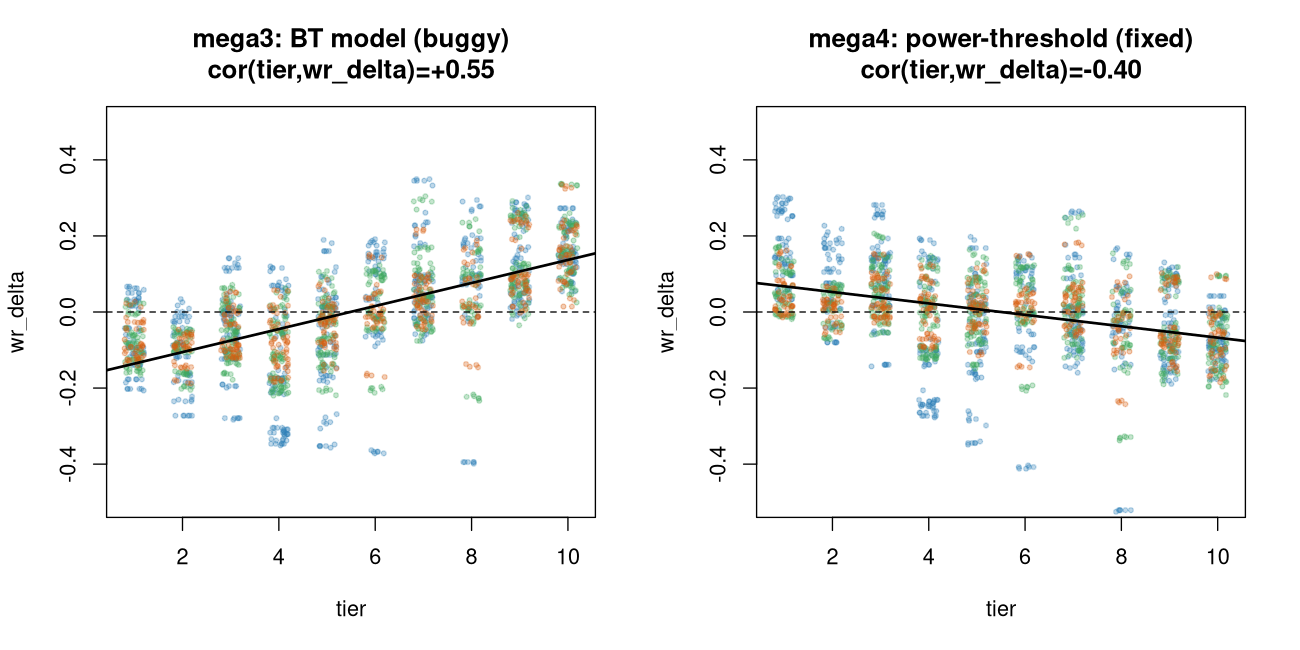
\includegraphics[width=0.86\linewidth,height=0.42\textheight,keepaspectratio]{plots/11_wrdelta_calibration_fix.png}
\caption*{\small expected\_wr calibration fix}
\end{figure}

\textbf{What \texttt{wr\_\allowbreak{}delta} actually measures.} Power \texttt{P} is a \textbf{fixed design target} assigned to each piece --- it does not move. Pieces are tuned (active/passive abilities + stat fine-tuning) so that each one's *realized* combat strength matches its assigned \texttt{P}. The corrected \texttt{expected\_\allowbreak{}wr} is the win rate a piece *should* post if it exactly hit its \texttt{P} target against the field it faced. Therefore:\\

\begin{quotebox}
\textbf{\texttt{wr\_\allowbreak{}delta} is the per-piece tuning residual.} \texttt{wr\_\allowbreak{}delta $\approx$ 0} $\rightarrow$ the piece is tuned on-target. \texttt{wr\_\allowbreak{}delta < 0} $\rightarrow$ \textbf{under-tuned} (its kit delivers less than its \texttt{P} promises). \texttt{wr\_\allowbreak{}delta > 0} $\rightarrow$ \textbf{over-tuned} (kit over-delivers vs \texttt{P}). The tuning goal is to drive every piece's \texttt{wr\_\allowbreak{}delta} toward 0 --- *not* to change \texttt{P}.
\end{quotebox}

The buggy BT model produced \texttt{cor(\allowbreak{}tier,\allowbreak{} wr\_\allowbreak{}delta)\allowbreak{} = +\allowbreak{}0.\allowbreak{}55$\rightarrow$+\allowbreak{}0.\allowbreak{}74}. Under the fixed power-threshold model the correlation \textbf{flips to −0.40} (stable across all three stages) and the spread tightens (\texttt{sd(\allowbreak{}wr\_\allowbreak{}delta)\allowbreak{}} 0.160$\rightarrow$0.147 in 1v1, 0.107$\rightarrow$0.074 in 3v3). The corrected reading:\\

\begin{itemize}
\item \textbf{There is a mild systematic under-tuning at high tiers.} The negative slope says high-\texttt{P} pieces realize *slightly less* than their target (their bigger kits don't fully cash in) while low-\texttt{P} pieces slightly over-deliver. It's a small residual, not an emergency --- but it points tuning effort toward the top of the roster.
\item \textbf{\texttt{power(\allowbreak{})\allowbreak{}} does not need re-fitting.} \texttt{P} is the fixed yardstick by design; the earlier "re-fit \texttt{power(\allowbreak{})\allowbreak{}}" idea was backwards. The lever is each piece's abilities/stats, measured *against* \texttt{P}.
\item \textbf{The tier \texttt{win\_\allowbreak{}rate} cliff is intended, not a bug} (\texttt{cor(\allowbreak{}tier,\allowbreak{} win\_\allowbreak{}rate)\allowbreak{} = 0.\allowbreak{}87}): a high-\texttt{P} piece *should* beat a low-\texttt{P} one. \S{}6's cliff is by-design decisiveness; only its old \texttt{wr\_\allowbreak{}delta} gloss was wrong.
\end{itemize}

\textbf{Corrected outlier reading (refines \S{}11):} with a trustworthy \texttt{wr\_\allowbreak{}delta}, the weak-mage list splits into two kinds ---\\

\medskip
\begin{tabularx}{\linewidth}{LL}
\toprule
\textbf{Genuine underperformers (lose vs equal/weaker power)} & \textbf{"Low but on budget" (just low-tier)} \\
\midrule
Hierarch T8 (−0.379), Marsh Thrush T6 (−0.264), Company Captain T5 (−0.209), Storm Eagle T9 (−0.158), Arcanist T9 (−0.111), Glade Heron T8 (−0.128) & Will-o-Fawn T2 (−0.069), Signal Drummer T1 (+0.009), Sparkfly T1 (+0.019), Dusk Bat T2 (−0.039) \\
\bottomrule
\end{tabularx}
\medskip

In tuning-target terms: the red column = mages whose kits are \textbf{under-tuned vs their assigned \texttt{P}} (they have the target strength to win and don't); the grey = mages that are \textbf{on-target} and simply low-\texttt{P}. This \textbf{sharpens the mage verdict (\S{}5):} the tuning work is concentrated in \textbf{mid/high-tier mages} (Hierarch T8 −0.38, Marsh Thrush T6 −0.26, Company Captain T5 −0.21, Storm Eagle/Arcanist T9) --- buff their abilities until \texttt{wr\_\allowbreak{}delta $\rightarrow$ 0}. The tier-1/2 mages (incl. Will-o-Fawn, the headline "0.05" piece) are mostly on-target --- their low win rate is their low \texttt{P}, not a tuning fault. \textbf{Mage fix priority = T6+ casters (Hierarch first), not the T1 floor.}\\

\begin{figure}[H]\centering
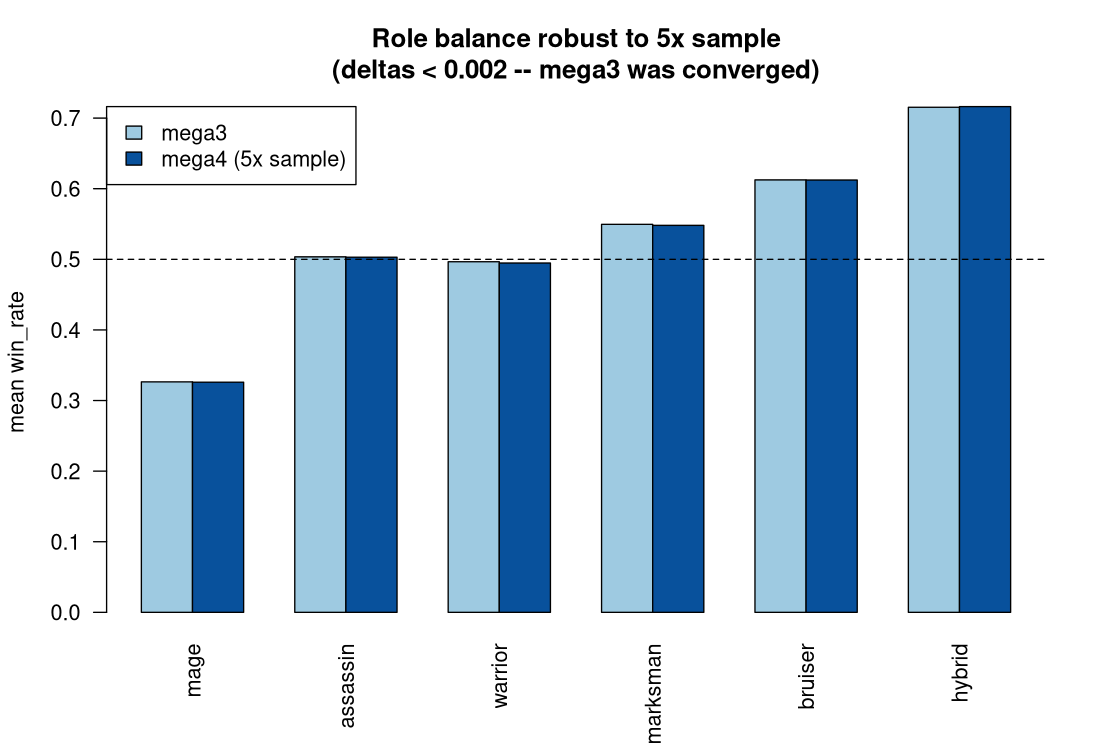
\includegraphics[width=0.86\linewidth,height=0.42\textheight,keepaspectratio]{plots/12_role_m3_vs_m4.png}
\caption*{\small role balance robust to 5x sample}
\end{figure}
\begin{figure}[H]\centering
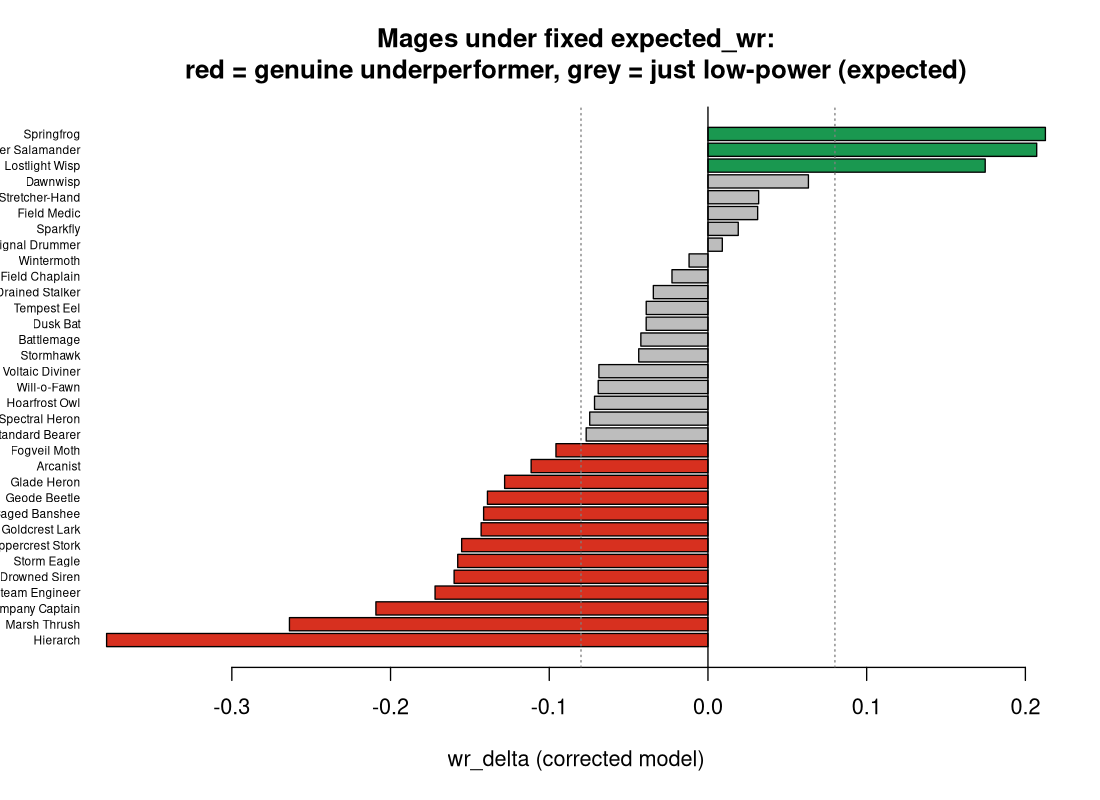
\includegraphics[width=0.86\linewidth,height=0.42\textheight,keepaspectratio]{plots/13_mage_fixed_model.png}
\caption*{\small mage under fixed model}
\end{figure}

Also note \textbf{Grand Marshal}: his \texttt{wr\_\allowbreak{}delta} drops from +0.31 (buggy) to \textbf{+0.07} (fixed) --- the threshold model correctly *expects* a T10 to win \textasciitilde{}0.96, so he's no longer a model-flagged overperformer. He is still a raw outlier (0.97 win, near-unloseable) and still worth a nerf; he's just winning about what his power says he should.\\


\section*{1. Dataset and method}

\medskip
\begin{tabularx}{\linewidth}{Lrrrr}
\toprule
\textbf{Stage} & \textbf{Weathers} & \textbf{Battles / weather} & \textbf{Pieces} & \textbf{Rated rows} \\
\midrule
1v1 (round-robin) & 6 & 7,140 & 120 & 720 \\
team2-sample (2v2) & 6 & 26,000 & 120 & 720 \\
team3-sample (3v3) & 6 & 16,000 & 120 & 720 \\
\bottomrule
\end{tabularx}
\medskip

\begin{itemize}
\item \textbf{294,840 battles} total across 18 \texttt{results\_\allowbreak{}*.\allowbreak{}csv}; \textbf{2,160 rated rows} (120 pieces $\times$ 3 stages $\times$ 6 weathers) across 18 \texttt{ratings\_\allowbreak{}*.\allowbreak{}csv}. (Mega4 re-runs the same design at \textasciitilde{}5$\times$ sample --- team2 130k/wx, team3 78k/wx --- see \S{}0.5.)
\item 120 pieces = 60 champions + 60 enemies. Affinity split is unbalanced by design: \textbf{clear 40, all others 16} (clear is the neutral default).
\item \textbf{\texttt{-\allowbreak{}-\allowbreak{}max-\allowbreak{}ticks 12000}} this run (vs mega2's effectively-infinite 1e6) $\rightarrow$ \textbf{timeouts now exist} (\textasciitilde{}11--13\% of fights). Every timeout is recorded as a \texttt{draw} (verified: \texttt{draw == timed\_\allowbreak{}out} to the row in all stages). This is the main reason duration/timeout metrics are *not* comparable to mega2.
\item \textbf{Metrics:} \texttt{win\_\allowbreak{}rate}; \texttt{expected\_\allowbreak{}wr}; \texttt{wr\_\allowbreak{}delta = win\_\allowbreak{}rate − expected\_\allowbreak{}wr}; \texttt{timeout\_\allowbreak{}rate}; \texttt{mean\_\allowbreak{}duration\_\allowbreak{}ticks}. \textbf{\texttt{expected\_\allowbreak{}wr} differs by run:} mega3 used a Bradley-Terry budget (since shown buggy --- it also emitted \texttt{beta}/\texttt{beta\_\allowbreak{}ratio}/\texttt{beta\_\allowbreak{}deviation\_\allowbreak{}pct}); \textbf{mega4 uses the corrected deterministic power-threshold model} (\S{}0.5). Read \texttt{wr\_\allowbreak{}delta} only from mega4.
\item \textbf{Power proxy} for the win-curve: team \texttt{$\Sigma$P} via \texttt{power(\allowbreak{}tier,\allowbreak{} 1)\allowbreak{}} mirroring src/game/scaling.py. Per-battle level isn't logged, so this is a level-1 proxy --- adds scatter, preserves monotone shape.
\end{itemize}


\section*{2. Aggregate balance is healthy}

Champion vs enemy mean win rate, symmetric and centered everywhere:\\

\medskip
\begin{tabularx}{\linewidth}{Lrr}
\toprule
\textbf{stage} & \textbf{champion} & \textbf{enemy} \\
\midrule
1v1 & 0.516 & 0.484 \\
2v2 & 0.508 & 0.494 \\
3v3 & 0.500 & 0.501 \\
\bottomrule
\end{tabularx}
\medskip

The \textasciitilde{}1.6pp champion edge in 1v1 dissolves with team size. Faction-level balance is \textbf{not} a problem. Every issue below lives *inside* the roster.\\

\begin{figure}[H]\centering
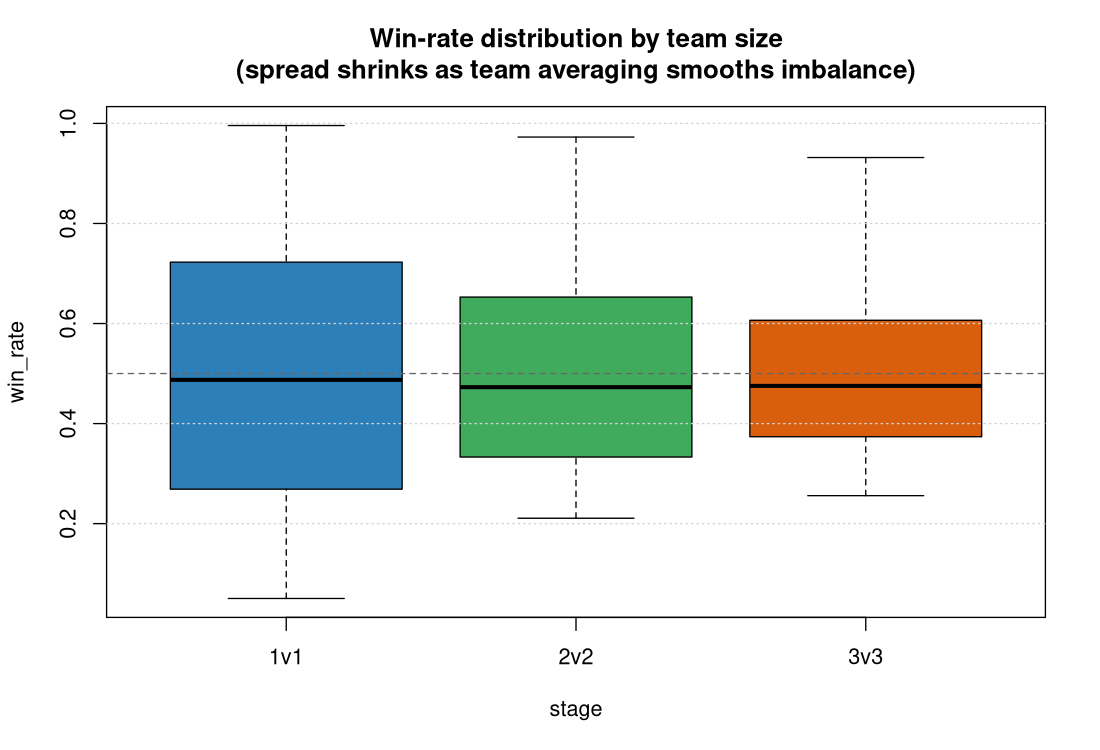
\includegraphics[width=0.86\linewidth,height=0.42\textheight,keepaspectratio]{plots/01_winrate_dist_by_stage.png}
\caption*{\small win-rate distribution by stage}
\end{figure}

The distribution \textbf{tightens dramatically with team size} --- \texttt{sd(\allowbreak{}win\_\allowbreak{}rate)\allowbreak{}} falls 0.267 (1v1) $\rightarrow$ 0.187 (2v2) $\rightarrow$ 0.149 (3v3). (Model-independent, so unaffected by the \texttt{expected\_\allowbreak{}wr} fix.) Team averaging launders individual imbalance: a broken piece on a 3-stack is diluted by two teammates. This is structural and matches mega2.\\


\section*{3. The kit-implementation flip (mega2 $\rightarrow$ mega3)}

Mega2's rectification note warned that the role verdicts were artifacts of the INT-scaled fallback nuke (\texttt{raw = 0.\allowbreak{}2$\cdot$STR +\allowbreak{} 4.\allowbreak{}2$\cdot$INT}, INT 21$\times$ STR). Mega3 confirms the warning \textbf{and} the predicted direction of correction:\\

\begin{figure}[H]\centering
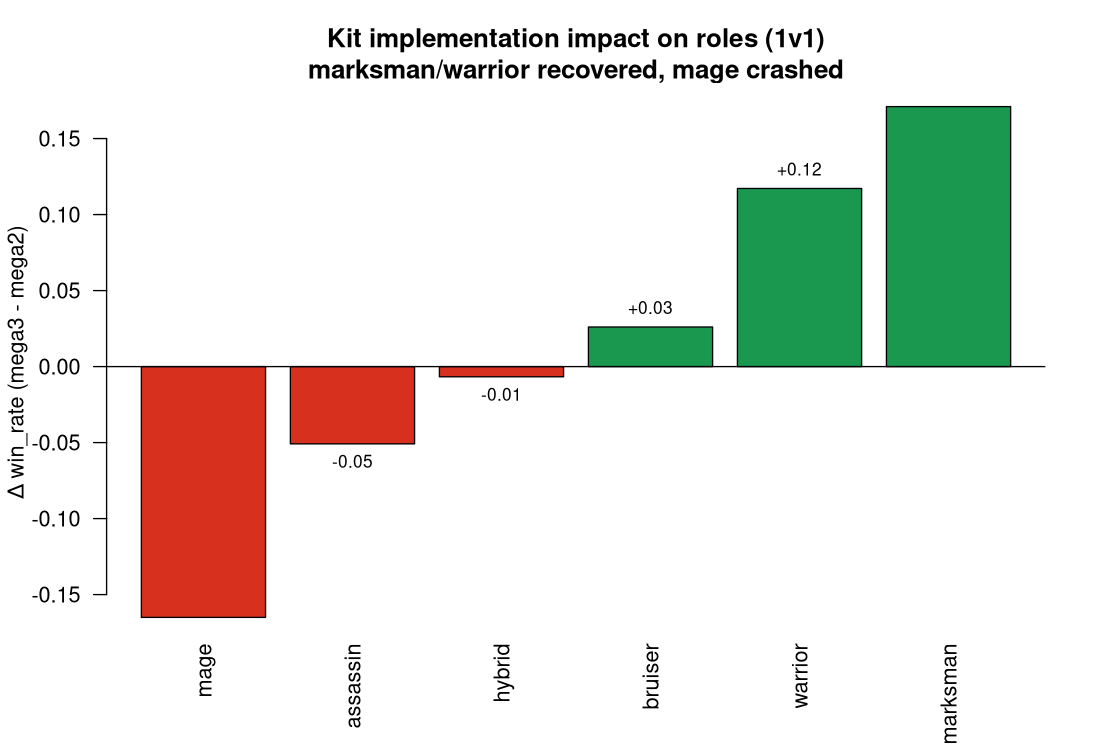
\includegraphics[width=0.86\linewidth,height=0.42\textheight,keepaspectratio]{plots/05_mega2_vs_mega3_role.png}
\caption*{\small mega2 vs mega3 role impact}
\end{figure}

\medskip
\begin{tabularx}{\linewidth}{LrrL}
\toprule
\textbf{role} & \textbf{mega2 (1v1)} & \textbf{mega3 (1v1)} & \textbf{$\Delta$} \\
\midrule
\textbf{marksman} & 0.374 & 0.545 & \textbf{+0.171} \\
\textbf{warrior} & 0.395 & 0.513 & \textbf{+0.117} \\
bruiser & 0.598 & 0.625 & +0.026 \\
hybrid & 0.782 & 0.776 & −0.007 \\
assassin & 0.594 & 0.544 & −0.051 \\
\textbf{mage} & 0.421 & 0.256 & \textbf{−0.165} \\
\bottomrule
\end{tabularx}
\medskip

STR/AD pieces (marksman, warrior) --- "crippled by the INT fallback, not mis-designed" per mega2 --- \textbf{recovered to \textasciitilde{}parity} the moment their real kits fired. But mage, which the fallback had been silently carrying, \textbf{fell off a cliff} once it had to rely on its actual kit. The fix was correct; the mage kit catalog is the new gap.\\


\section*{4. Role balance --- tier-confounded; mage \& hybrid under-deliver, marksman/warrior over-deliver}

\begin{figure}[H]\centering
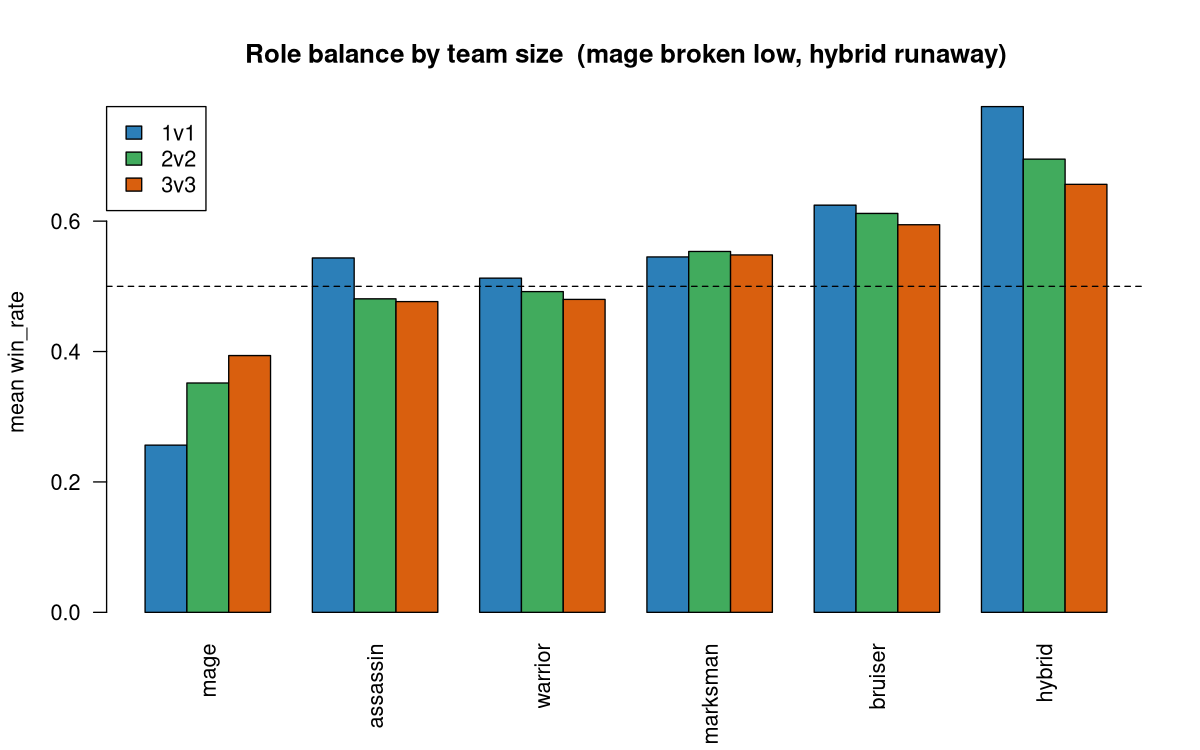
\includegraphics[width=0.86\linewidth,height=0.42\textheight,keepaspectratio]{plots/02_role_balance.png}
\caption*{\small role balance by stage}
\end{figure}

\begin{quotebox}
\textbf{[!]} \textbf{Read raw role \texttt{win\_\allowbreak{}rate} with care --- it is confounded by tier.} Roles are not evenly spread across tiers: mage mean tier \textbf{4.1}, hybrid mean tier \textbf{9.1} (median 10). So "mage lowest / hybrid highest win\_rate" largely restates "mage pieces are low-tier, hybrid pieces are high-tier." The honest role signal is the \textbf{corrected \texttt{wr\_\allowbreak{}delta}} (delivery vs the \texttt{P} target, \S{}0.5) and the \textbf{within-tier} comparison below.
\end{quotebox}

Overall mean win rate (raw) and \textbf{corrected (mega4) \texttt{wr\_\allowbreak{}delta}} by role:\\

\medskip
\begin{tabularx}{\linewidth}{LrrLL}
\toprule
\textbf{role} & \textbf{win\_rate} & \textbf{mean tier} & \textbf{\texttt{wr\_\allowbreak{}delta} (corrected)} & \textbf{reading} \\
\midrule
\textbf{mage} & 0.334 & 4.1 & \textbf{−0.064} & low win = low tier; under-delivers, worst at high tier (\S{}5) \\
assassin & 0.500 & 5.9 & −0.014 & on-target \\
warrior & 0.495 & 4.5 & \textbf{+0.072} & \textbf{over-target} (wins more than \texttt{P} warrants) \\
marksman & 0.549 & 5.0 & \textbf{+0.087} & \textbf{most over-target} \\
bruiser & 0.610 & 6.5 & +0.041 & mildly over-target \\
\textbf{hybrid} & \textbf{0.709} & \textbf{9.1} & \textbf{−0.082} & **most *under*-target --- high win\_rate is pure tier** \\
\bottomrule
\end{tabularx}
\medskip

The corrected \texttt{wr\_\allowbreak{}delta} ranking is \textbf{nearly the reverse} of the raw-win\_rate ranking. Two reframes follow:\\

\begin{itemize}
\item **Hybrid is *not* a runaway over-powered role.\textbf{ Its 0.71 win\_rate is a roster-composition artifact: hybrids are almost all tier 9--10. }Within tier, hybrids win 6--9pp *less* than non-hybrids at the same tier** ($\Delta$ = −0.057 to −0.091; mean −0.082) --- they *under*-deliver their \texttt{P}, the same direction as mage. No nerf is warranted; if anything hybrid kits are slightly under-tuned. *(The earlier "hybrid runaway / design debt" read was an un-tier-controlled error.)*
\item \textbf{The genuinely over-target roles are marksman (+0.087) and warrior (+0.072)} --- they win more than their (lower) \texttt{P} says they should. If any role is "too strong for its power," it's these two, not hybrid.
\end{itemize}

So the under-delivering roles (buff candidates) are \textbf{mage and hybrid}; the over-delivering roles (trim candidates) are \textbf{marksman and warrior}; assassin/bruiser are close to on-target. Mage stays the priority because its under-delivery concentrates in expensive high-tier casters (\S{}5) and it also owns the raw-win\_rate floor.\\


\section*{5. Mage deep-dive --- the diagnosis}

\begin{figure}[H]\centering
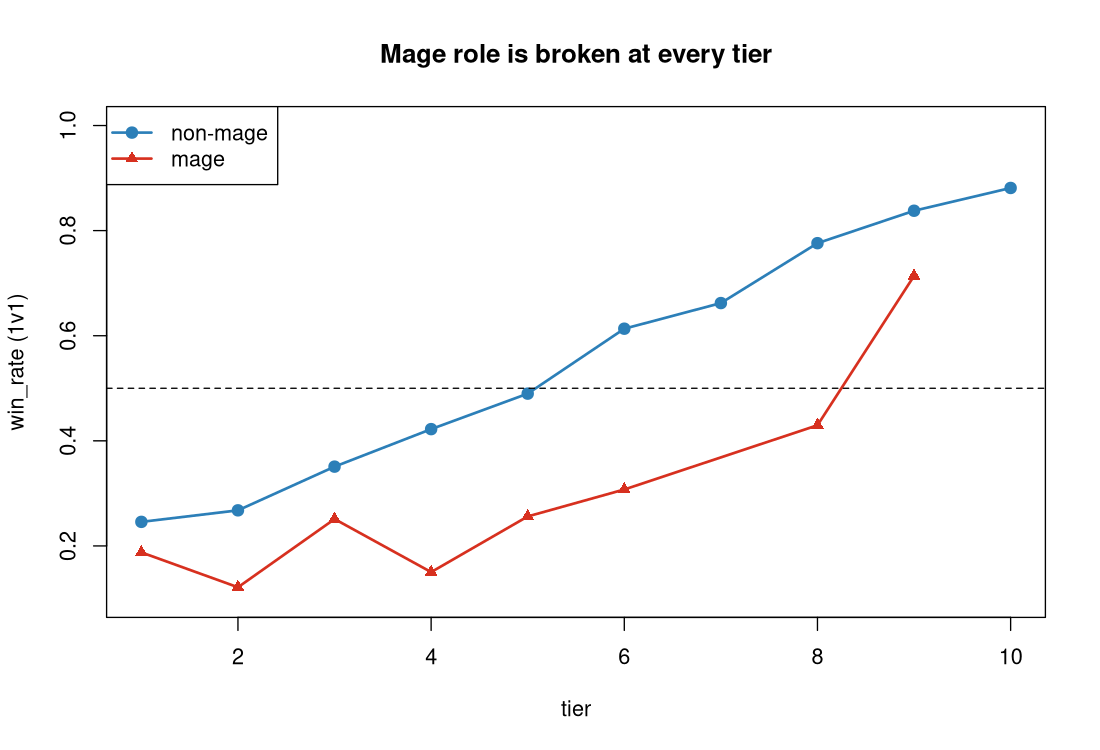
\includegraphics[width=0.86\linewidth,height=0.42\textheight,keepaspectratio]{plots/09_mage_deepdive.png}
\caption*{\small mage vs non-mage by tier}
\end{figure}

The mage line tracks \textasciitilde{}0.15--0.25 *below* non-mages at \textbf{every} tier. A tier-9 mage barely reaches parity; the roster has no tier-10 mage to test the ceiling.\\

Controls that rule out the easy explanations:\\

\begin{itemize}
\item \textbf{Not a faction bug.} Mage champions (0.355) and mage enemies (0.309) are *both* broken. It is the role, not one content author.
\item \textbf{Not a tier artifact.} Mean within-tier deficit vs non-mages (1v1) = \textbf{0.198}. Even matched on tier, a mage loses \textasciitilde{}20pp it shouldn't.
\item \textbf{Mechanism = no burst, no bulk.} Mages have the lowest HP and now lack the free INT nuke that the fallback gave everyone. Their fights run *longer* than average (7157 vs 6954 ticks in 1v1) and they still lose --- they neither kill fast nor survive. timeout\_rate (0.15) is mid-pack: they don't stall to a draw, they get ground out.
\end{itemize}

\textbf{This is the report's top action item.} The mage kit catalog either deals too little damage, fires too slowly, or both. Re-tune mage abilities (burst windows / cast cadence / base HP) and re-sim before any other balance pass.\\


\section*{6. The tier cliff}

\begin{figure}[H]\centering
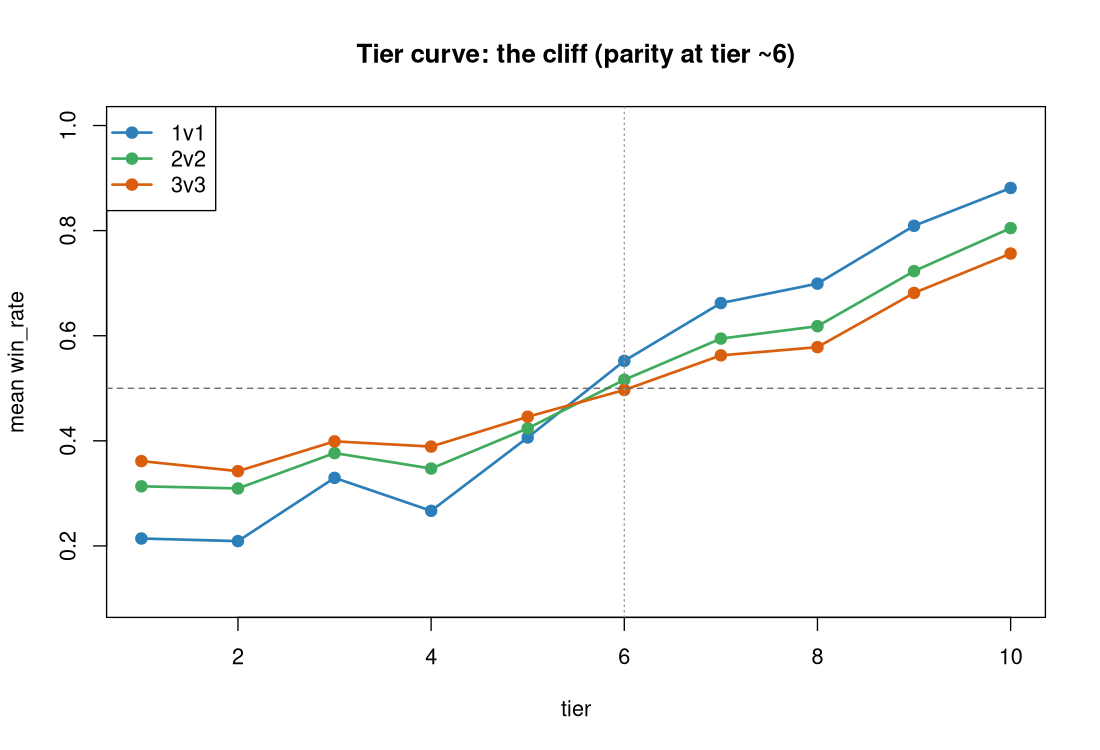
\includegraphics[width=0.86\linewidth,height=0.42\textheight,keepaspectratio]{plots/03_tier_curve.png}
\caption*{\small tier curve}
\end{figure}

The cliff that dominated mega2 \textbf{survived the kit rewrite intact}. \texttt{cor(\allowbreak{}tier,\allowbreak{} win\_\allowbreak{}rate)\allowbreak{} $\approx$ 0.\allowbreak{}87} in all three stages. Parity crosses at \textbf{tier \textasciitilde{}6}: tiers 1--5 are net losers, 7--10 net winners. The low-tier floor is brutal --- tier-1/2 pieces win \textasciitilde{}21\% in 1v1. This is an observed-outcome fact, independent of any rating model, and it is \textbf{confirmed unchanged at mega4's 5$\times$ sample.}\\

\begin{quotebox}
\textbf{[!]} \textbf{Corrected --- see \S{}0.5.} This section originally argued from \texttt{wr\_\allowbreak{}delta} that "high tiers beat their power budget" (\texttt{cor(\allowbreak{}tier,\allowbreak{} wr\_\allowbreak{}delta)\allowbreak{} = +\allowbreak{}0.\allowbreak{}55$\rightarrow$+\allowbreak{}0.\allowbreak{}74}) and that \texttt{power(\allowbreak{})\allowbreak{}} under-rewards low tiers. \textbf{That rested on a buggy \texttt{expected\_\allowbreak{}wr}.} Under mega4's fixed power-threshold model the correlation flips to \textbf{−0.40} and the spread tightens --- there is *no* systematic under-reward of low tiers. The \texttt{power(\allowbreak{})\allowbreak{}} curve does \textbf{not} need re-fitting. The cliff is about HP/DPS/focus-fire decisiveness (\S{}7), not a scaling-math error. The plot below (\texttt{06\_\allowbreak{}wrdelta\_\allowbreak{}vs\_\allowbreak{}tier.\allowbreak{}png}, buggy metric) is retained only for the before/after in \S{}0.5.
\end{quotebox}


\section*{7. Decisiveness and the win-curve}

\begin{figure}[H]\centering
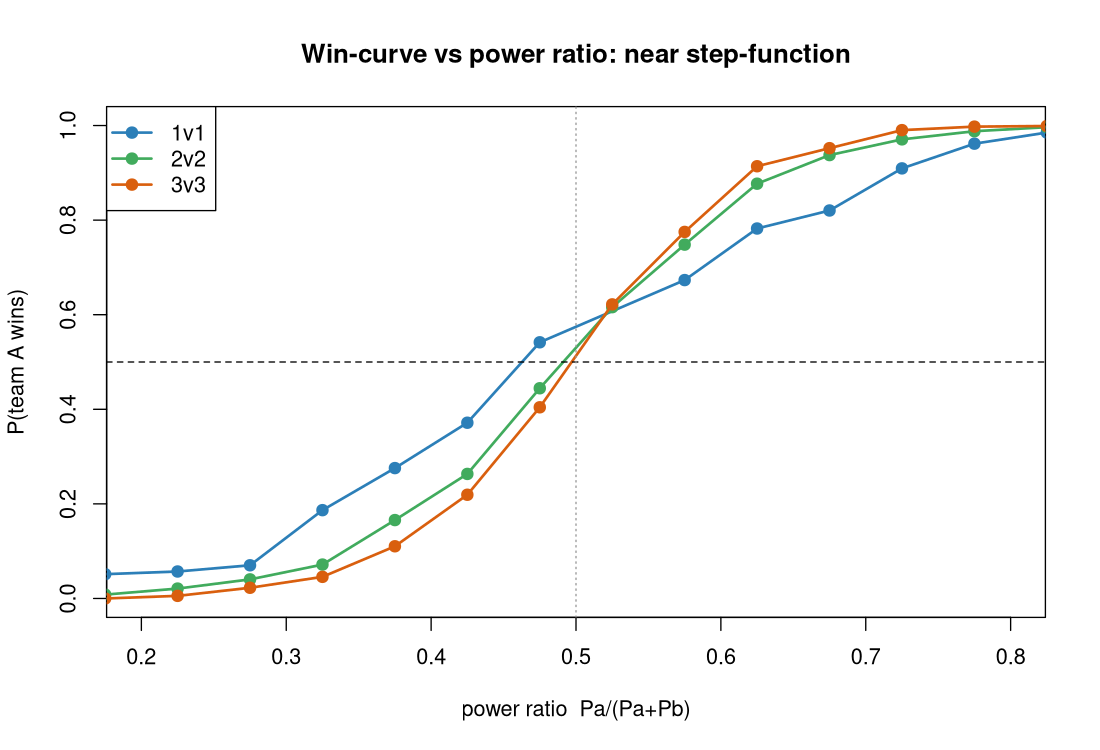
\includegraphics[width=0.86\linewidth,height=0.42\textheight,keepaspectratio]{plots/04_wincurve_powerratio.png}
\caption*{\small win-curve vs power ratio}
\end{figure}

Combat is still a \textbf{near step-function} of power ratio --- the contested band (where P(win) $\in$ [0.2, 0.8]) is roughly \texttt{Pa/\allowbreak{}(\allowbreak{}Pa+\allowbreak{}Pb)\allowbreak{} $\in$ [0.\allowbreak{}35,\allowbreak{} 0.\allowbreak{}65]}. Two refinements over mega2:\\

\begin{itemize}
\item \textbf{3v3 is the steepest} (most decisive at parity), 1v1 the flattest. More bodies $\rightarrow$ more reliable focus-fire $\rightarrow$ less variance $\rightarrow$ sharper curve. Consistent with the \texttt{sd(\allowbreak{}win\_\allowbreak{}rate)\allowbreak{}} shrink in \S{}2.
\item \textbf{1v1 carries a side-A bias.} The 1v1 curve crosses 0.5 *left* of parity; at \texttt{|pr−0.\allowbreak{}5|<0.\allowbreak{}025}, side A wins \textbf{0.542} in 1v1 vs \textasciitilde{}0.51 in 2v2/3v3. A \textasciitilde{}4pp initiative/turn-order advantage in duels. Worth checking the 1v1 tie-break / who-acts-first logic.
\end{itemize}

Winner HP-remaining (stomp proxy) scales with team size --- 799 (1v1) / 1406 (2v2) / 1937 (3v3) --- i.e. larger fights end with more leftover HP on the winning side: snowball/focus-fire leaves survivors at high HP.\\

\textbf{Balance scorecard} (fraction of piece$\times$stage$\times$weather cells near parity):\\

\medskip
\begin{tabularx}{\linewidth}{Lrrr}
\toprule
\textbf{stage} & \textbf{in [.45,.55]} & \textbf{blowout <.3} & \textbf{blowout >.7} \\
\midrule
1v1 & 0.11 & 0.28 & 0.28 \\
2v2 & 0.17 & 0.14 & 0.18 \\
3v3 & 0.25 & 0.04 & 0.12 \\
\bottomrule
\end{tabularx}
\medskip

1v1 is \textbf{highly polarized} --- only 11\% of matchups are competitive, 56\% are blowouts. This is the cliff (\S{}6) plus the role tails (\S{}4) compounding. It tightens at 3v3 but never gets *good*.\\


\section*{8. Weather is nearly inert}

The signature mechanic --- real-world weather shaping combat --- barely registers.\\

\begin{figure}[H]\centering
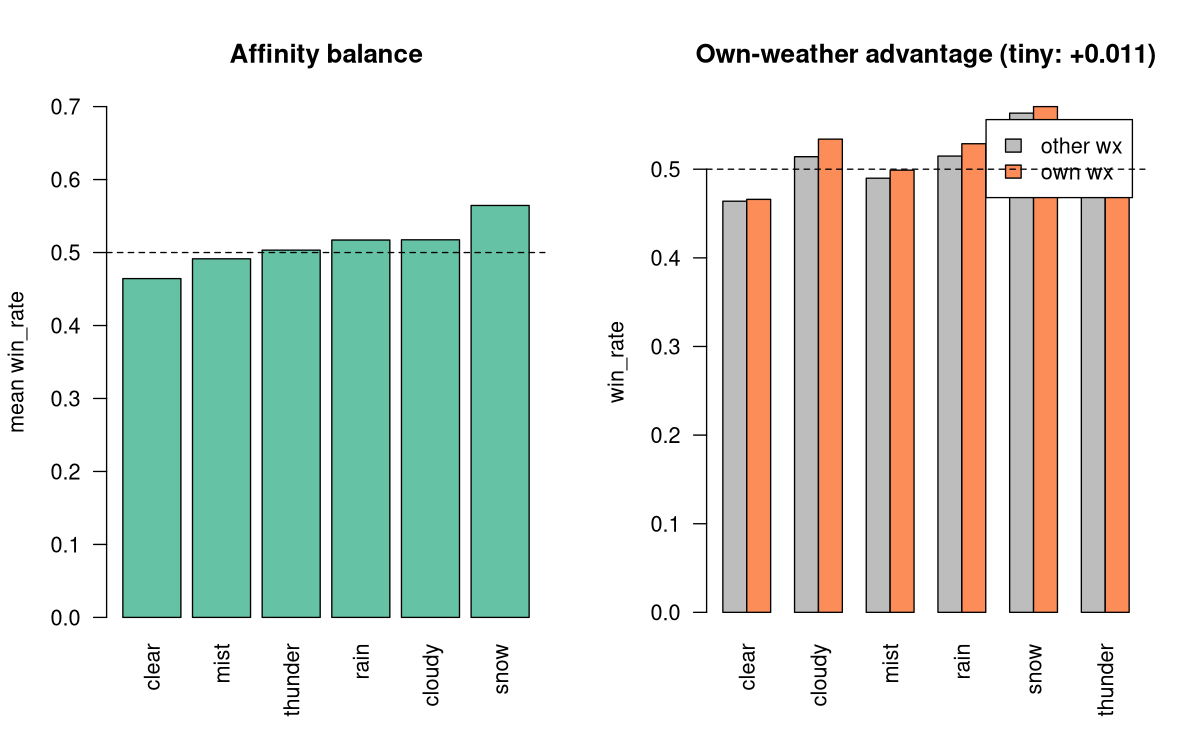
\includegraphics[width=0.86\linewidth,height=0.42\textheight,keepaspectratio]{plots/08_affinity.png}
\caption*{\small affinity balance and own-weather effect}
\end{figure}

\begin{itemize}
\item \textbf{Own-weather advantage = +0.011 win rate.} A piece fighting in its own affinity-weather wins 0.509 vs 0.499 otherwise. Largest sub-effect is thunder (+0.024); clear is \textasciitilde{}0.
\item \textbf{Mean per-piece win-rate range across all 6 weathers = 0.027} (median 0.022). The *most* weather-sensitive piece (Aerion) swings only 0.090.
\item \textbf{Smoking gun:} Grand Marshal posts an *identical* 0.9958 in clear, cloudy, mist, and rain (\S{}11). Will-o-Fawn posts an identical 0.0504 across mist/rain/snow/thunder. Outcomes are weather-invariant to 4 decimals for the pieces where it would matter most.
\end{itemize}

Either the weather stat-packs / affinity damage-triangle apply tiny coefficients, or kits don't read weather state. For a game whose pitch is "live weather shapes combat," a $\pm$1pp effect is a thematic failure. \textbf{Recommend a dedicated weather-sensitivity audit} before shipping --- this is a top-3 issue even though it isn't a *balance* issue.\\


\section*{9. Affinity balance}

\texttt{wr\_\allowbreak{}delta} shown is the \textbf{corrected (mega4)} value:\\

\medskip
\begin{tabularx}{\linewidth}{LrLr}
\toprule
\textbf{affinity} & \textbf{win\_rate} & \textbf{\texttt{wr\_\allowbreak{}delta} (corrected)} & \textbf{n pieces} \\
\midrule
clear & 0.464 & +0.010 & 40 \\
mist & 0.491 & −0.033 & 16 \\
thunder & 0.503 & −0.023 & 16 \\
rain & 0.517 & −0.007 & 16 \\
cloudy & 0.517 & −0.005 & 16 \\
snow & 0.564 & +0.042 & 16 \\
\bottomrule
\end{tabularx}
\medskip

Spread is modest (win\_rate 0.46--0.56). \textbf{Snow runs hot} on both metrics (+0.042 over target). Under the corrected model, \textbf{clear is actually on-target} (+0.010) --- its low win\_rate is just its low-tier-heavy roster (40 pieces incl. most low-tier mages), not a tuning fault; \textbf{mist/thunder mildly under-deliver} (−0.03/−0.02). All second-order next to mage/tier/weather. *(Note the sign flip vs the buggy mega3 values --- clear was −0.016, now +0.010.)*\\


\section*{10. Stalemates and timeouts}

With \texttt{-\allowbreak{}-\allowbreak{}max-\allowbreak{}ticks 12000}, \textasciitilde{}11--13\% of fights now time out ($\rightarrow$ draw). Distribution by role:\\

\medskip
\begin{tabularx}{\linewidth}{Lr}
\toprule
\textbf{role} & \textbf{timeout\_rate} \\
\midrule
bruiser & 0.239 \\
mage & 0.150 \\
warrior & 0.116 \\
assassin & 0.114 \\
hybrid & 0.064 \\
marksman & 0.040 \\
\bottomrule
\end{tabularx}
\medskip

\begin{figure}[H]\centering
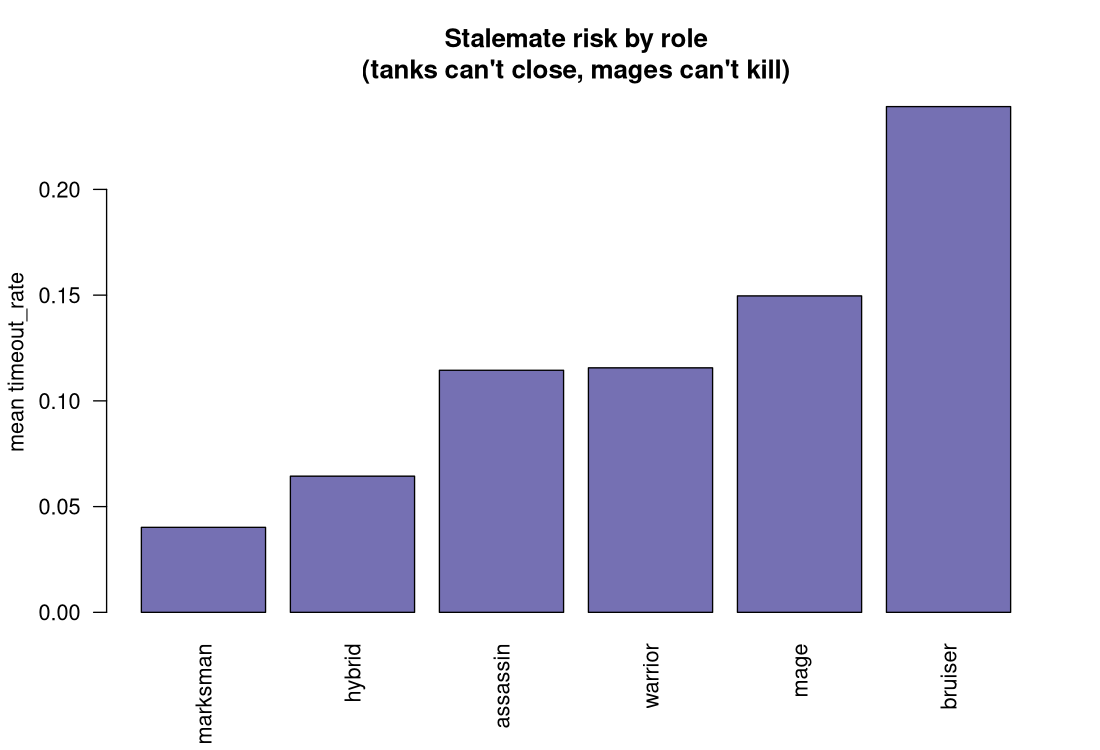
\includegraphics[width=0.86\linewidth,height=0.42\textheight,keepaspectratio]{plots/07_timeout_by_role.png}
\caption*{\small timeout by role}
\end{figure}

Two distinct stall modes: \textbf{tanks that can't close} (bruiser/warrior --- high HP, low burst $\rightarrow$ mutual attrition) and \textbf{mages that can't kill} (low damage). Marksman/hybrid resolve cleanly. The worst single piece is \textbf{Coral Colossus} (warrior T5, 46\% timeouts, mean 10,063 ticks) --- a damage-starved wall. Bruiser timeouts are the strongest argument for keeping a finite max-ticks + sudden-death rule rather than mega2's 1e6.\\


\section*{11. Outlier roster}

\textbf{Strongest (mean win\_rate, all stages/weathers):}\\

\medskip
\begin{tabularx}{\linewidth}{LLLrrr}
\toprule
\textbf{name} & \textbf{affinity} & \textbf{role} & \textbf{tier} & \textbf{win\_rate} & \textbf{wr\_delta} \\
\midrule
\textbf{Grand Marshal} & clear & warrior & 10 & \textbf{0.963} & \textbf{+0.311} \\
Storm Tyrant & thunder & hybrid & 10 & 0.882 & +0.228 \\
Aurion, the First Dawn & clear & hybrid & 10 & 0.882 & +0.228 \\
Sunspear Falcon & clear & marksman & 9 & 0.873 & +0.258 \\
Quarried Behemoth & cloudy & bruiser & 9 & 0.864 & +0.248 \\
Glacierback Mammoth & snow & bruiser & 7 & 0.828 & \textbf{+0.282} \\
\bottomrule
\end{tabularx}
\medskip

\textbf{Weakest --- every one is a mage:}\\

\medskip
\begin{tabularx}{\linewidth}{LLLrrL}
\toprule
\textbf{name} & \textbf{affinity} & \textbf{role} & \textbf{tier} & \textbf{win\_rate} & \textbf{wr\_delta} \\
\midrule
\textbf{Will-o-Fawn} & mist & mage & 2 & \textbf{0.176} & −0.218 \\
Steam Engineer & clear & mage & 4 & 0.198 & −0.247 \\
Signal Drummer & clear & mage & 1 & 0.205 & −0.162 \\
Dusk Bat & cloudy & mage & 2 & 0.216 & −0.179 \\
Coppercrest Stork & thunder & mage & 4 & 0.219 & −0.228 \\
Drowned Siren & rain & mage & 4 & 0.220 & −0.230 \\
\bottomrule
\end{tabularx}
\medskip

\begin{quotebox}
\textbf{[!]} \textbf{The \texttt{wr\_\allowbreak{}delta} column in both tables above uses the buggy mega3 metric.} For the trustworthy tuning-residual ranking, use the corrected values in \S{}0.5. \texttt{win\_\allowbreak{}rate} (raw outcome) is correct as shown.
\end{quotebox}

Specific flags (with corrected mega4 \texttt{wr\_\allowbreak{}delta}):\\

\begin{itemize}
\item \textbf{Hierarch} (clear mage T8) --- corrected \texttt{wr\_\allowbreak{}delta} = \textbf{−0.379}, the single most under-tuned piece in the roster: a high-\texttt{P} caster whose kit delivers nowhere near its target. \textbf{Top buff target.}
\item \textbf{Grand Marshal} --- hits \textbf{0.9685 overall / 0.9958 in 1v1, weather-invariant}, near-unloseable. But corrected \texttt{wr\_\allowbreak{}delta} is only \textbf{+0.07} --- he's winning roughly what his T10 \texttt{P} *says* he should. He's a "feels-bad invincible" UX problem more than a tuning-error problem; nerf only if his \texttt{P} target itself is meant to be lower.
\item \textbf{Marsh Thrush} (T6 mage, −0.264) / \textbf{Company Captain} (T5 mage, −0.209) --- next under-tuned casters after Hierarch.
\item \textbf{Glacierback Mammoth} (T7 bruiser) --- corrected \texttt{wr\_\allowbreak{}delta} $\approx$ +0.08, mildly over-target; minor trim at most (the buggy +0.282 over-stated it).
\item \textbf{Will-o-Fawn} --- 0.168 win, weather-invariant, but corrected \texttt{wr\_\allowbreak{}delta} $\approx$ −0.07: \textbf{on-target for its T2 \texttt{P}.} Not a tuning fault; previously mis-flagged as "bottom of the crisis."
\end{itemize}

\begin{figure}[H]\centering
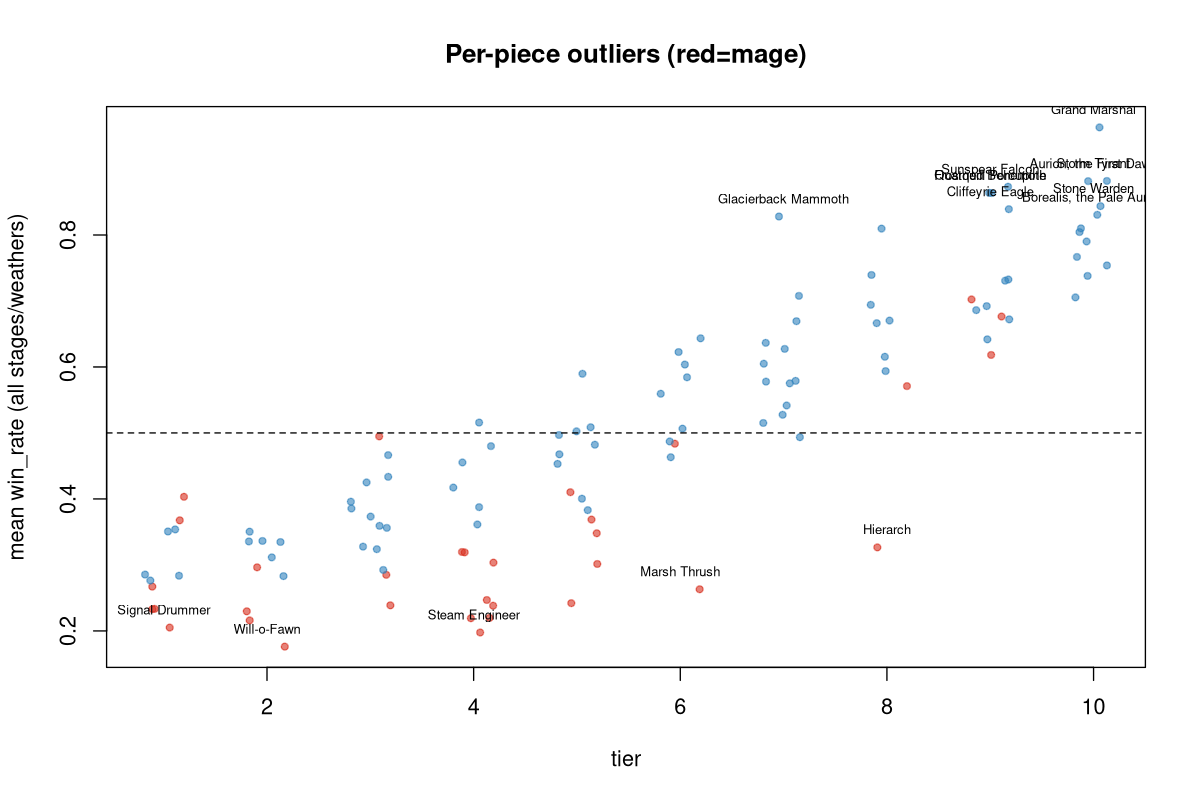
\includegraphics[width=0.86\linewidth,height=0.42\textheight,keepaspectratio]{plots/10_piece_outliers.png}
\caption*{\small per-piece outliers}
\end{figure}


\section*{12. Prioritized recommendations}

All recommendations are framed as \textbf{tuning pieces toward \texttt{wr\_\allowbreak{}delta $\rightarrow$ 0} against their fixed \texttt{P} targets} --- never as changing \texttt{P}.\\

\medskip
\begin{tabularx}{\linewidth}{rLLL}
\toprule
\textbf{\#} & \textbf{Action} & \textbf{Why} & \textbf{Effort} \\
\midrule
\textbf{1} & \textbf{Buff the mage kit catalog, T6+ first} (Hierarch, Marsh Thrush, Company Captain, Storm Eagle, Arcanist) & Mage is the one broken role (0.33, −0.20 within-tier, both factions, \S{}5); the corrected residual localises the fault to mid/high-tier casters that under-deliver vs \texttt{P} (\S{}0.5) & High \\
\textbf{2} & \textbf{Audit weather coefficients / confirm kits read weather} & Own-weather worth +0.008--0.011; outcomes weather-invariant to 4dp --- the core mechanic is inert (\S{}8) & Med \\
\textbf{3} & \textbf{Drive \texttt{|wr\_\allowbreak{}delta|} $\rightarrow$ 0 roster-wide; close the −0.40 high-tier under-tuning slope} & \texttt{wr\_\allowbreak{}delta} is the tuning-error signal vs the fixed \texttt{P} target; do \textbf{not} re-fit \texttt{power(\allowbreak{})\allowbreak{}} (\S{}0.5). High-\texttt{P} kits systematically under-deliver & Med \\
\textbf{4} & \textbf{Buff Hierarch (−0.38, most under-tuned piece)} & Largest single tuning residual in the roster (\S{}11) & Low \\
\textbf{5} & \textbf{Trim marksman \& warrior, or buff hybrid --- they're the real per-\texttt{P} outliers} & Corrected \texttt{wr\_\allowbreak{}delta}: marksman +0.087 / warrior +0.072 \textbf{over}-deliver; hybrid −0.082 \textbf{under}-delivers (its 0.71 win is just high tier). Hybrid is *not* over-powered (\S{}4) & Med \\
\textbf{6} & **Decide if Grand Marshal's *target* is correct** & 0.97 win / near-unloseable, but \texttt{wr\_\allowbreak{}delta}$\approx$+0.07 --- on-target. UX call, not a tuning bug (\S{}11) & Low \\
\textbf{7} & \textbf{Investigate 1v1 side-A bias (\textasciitilde{}4pp at parity)} & Initiative/turn-order edge in duels (\S{}7) & Low \\
\textbf{8} & \textbf{Keep finite max-ticks + add sudden-death} & Bruiser/warrior stalls hit 24\% timeout; mega2's 1e6 hid this (\S{}10) & Low \\
\bottomrule
\end{tabularx}
\medskip

Sequence: do \textbf{\#1} then re-sim. Don't trust hybrid/affinity verdicts until mage is fixed --- a broken role drags every opponent's win rate and distorts the field. Re-run a full mega (incl. team3 snow+thunder) after the mage buff and re-read \texttt{wr\_\allowbreak{}delta}.\\


\section*{13. What's trustworthy vs provisional}

\begin{itemize}
\item \textbf{Solid (structural), confirmed at mega4's 5$\times$ sample:} aggregate faction balance, the cliff, team-size variance shrink, the win-curve shape, the mage collapse (controlled for tier *and* faction), the kit-flip direction. \texttt{win\_\allowbreak{}rate} is \textbf{identical mega3$\leftrightarrow$mega4 in 1v1} (full round-robin, same battles); team2/team3 use freshly sampled matchups so they drift $\leq$0.002 --- still well within convergence.
\item \textbf{Now trustworthy (after the fix):} \texttt{wr\_\allowbreak{}delta} as a per-piece tuning residual vs the fixed \texttt{P} target. The mega3 \texttt{wr\_\allowbreak{}delta} numbers in \S{}6/\S{}11 were on the buggy metric --- use the \S{}0.5 corrected values.
\item \textbf{Provisional:} absolute role/affinity numbers shift once the mage kit is buffed (mage opponents' win rates are inflated by farming mages). \textbf{team3 mega4 is incomplete (4/6 weathers)} --- its \texttt{wr\_\allowbreak{}delta} will firm up when snow+thunder land.
\item \textbf{Caveat:} weather samples are sane but the +0.008--0.011 effect is small enough that any per-affinity number is within noise; treat \S{}9 as directional.
\end{itemize}


\section*{14. Reproducibility}

All scripts in \texttt{reviews/\allowbreak{}mega\_\allowbreak{}sim/\allowbreak{}}, base R only (no external packages):\\

\medskip
\begin{tabularx}{\linewidth}{LL}
\toprule
\textbf{script} & \textbf{output} \\
\midrule
\texttt{00\_\allowbreak{}load.\allowbreak{}R} & loader helpers (\texttt{power}, \texttt{load\_\allowbreak{}ratings(\allowbreak{}dir)\allowbreak{}}, \texttt{load\_\allowbreak{}results(\allowbreak{}dir)\allowbreak{}}, \texttt{team\_\allowbreak{}power}); schema-tolerant across mega3/mega4 \\
\texttt{01\_\allowbreak{}analysis.\allowbreak{}R} & core mega3 stats $\rightarrow$ \texttt{tables/\allowbreak{}*.\allowbreak{}csv}, \texttt{cache.\allowbreak{}rds} \\
\texttt{02\_\allowbreak{}results.\allowbreak{}R} & per-battle win-curve + mega2 comparison $\rightarrow$ \texttt{cache\_\allowbreak{}results.\allowbreak{}rds} \\
\texttt{03\_\allowbreak{}plots.\allowbreak{}R} & mega3 plots 01--10 $\rightarrow$ \texttt{plots/\allowbreak{}} \\
\texttt{04\_\allowbreak{}mega4.\allowbreak{}R} & mega4 load + corrected-model stats + mega3$\leftrightarrow$mega4 comparison $\rightarrow$ \texttt{cache\_\allowbreak{}mega4.\allowbreak{}rds} \\
\texttt{05\_\allowbreak{}mega4\_\allowbreak{}plots.\allowbreak{}R} & corrected-model plots 11--13 $\rightarrow$ \texttt{plots/\allowbreak{}} \\
\bottomrule
\end{tabularx}
\medskip

\begin{lstlisting}
cd /home/merlindk/development/tempest-fauna-trail
Rscript reviews/mega_sim/01_analysis.R     # mega3 core
Rscript reviews/mega_sim/02_results.R      # mega3 win-curve + mega2 cmp
Rscript reviews/mega_sim/03_plots.R        # mega3 plots
Rscript reviews/mega_sim/04_mega4.R        # mega4 + corrected expected_wr
Rscript reviews/mega_sim/05_mega4_plots.R  # calibration-fix plots
\end{lstlisting}

Tables: \texttt{tables/\allowbreak{}\{\allowbreak{}role\_\allowbreak{}balance,\allowbreak{}affinity\_\allowbreak{}balance,\allowbreak{}tier\_\allowbreak{}curve,\allowbreak{}weather\_\allowbreak{}sensitivity,\allowbreak{}piece\_\allowbreak{}overall,\allowbreak{}wincurve,\allowbreak{}mega2\_\allowbreak{}vs\_\allowbreak{}mega3\_\allowbreak{}role,\allowbreak{}mega3\_\allowbreak{}vs\_\allowbreak{}mega4\_\allowbreak{}role,\allowbreak{}mega4\_\allowbreak{}piece\_\allowbreak{}overall\}\allowbreak{}.\allowbreak{}csv}.\\

\textbf{Note on mega4 schema:} mega4 ratings dropped the Bradley-Terry columns (\texttt{beta}, \texttt{beta\_\allowbreak{}ratio}, \texttt{beta\_\allowbreak{}deviation\_\allowbreak{}pct}) when \texttt{expected\_\allowbreak{}wr} moved to the deterministic power-threshold model. \texttt{00\_\allowbreak{}load.\allowbreak{}R} handles both via \texttt{load\_\allowbreak{}ratings(\allowbreak{}dir,\allowbreak{} common=TRUE)\allowbreak{}}.\\

\end{document}